\subsection{Backend}

\subsubsection{Využité technologie}
Jako stavební kámen pro backendovou část je použit Node.js s frameworkem Express.js. Na samotném Expressu běží GraphQL, které se stará o dotazy. Dále je zde také zaregistrován zpracovatel dotazů pro GraphQL Subscription který zodpovídá za komunikaci v reálném čase.\par
Při použití jednoho serveru by bylo možné provozovat GraphQL Subscription pouze pomocí paměti tohoto jednoho serveru. Pokud bychom však chtěli rozdělit zátěž mezi více serverů, hrozilo by riziko, že dojde k desynchronizaci stavu kontrolérové části a frontendové části (například: Frontend si vytvořil komunikaci mezi sebou a serverem číslo 1. Další dotaz z kontroléru přišel na server 2, server tomuto zařízení odpověděl zpět bez problému, ale nebyl schopen oznámit frontendu o tom, že se něco stalo, protože tyto 2 servery o sobě navzájem neví). Proto je potřeba využít funkci Redisu s názvem Pub/Sub\cite{PubSub}, která oznámí změnu stavu všem podřízeným serverům.\par
Jako databáze byla zvolena databáze MongoDB, kvůli možnosti zpracovávat velké množství dat. Pro propojení backendu a databáze byla použita Prisma. Na dotazy, které by se často opakovaly, by nebylo exektivní se stále dokola dotazovat databáze, proto se určité, často opakované dotazy ukládají do cache paměti Redis.\par

\subsubsection{Autorizace}
Pro přístup k většině dotazů je potřeba být přihlášen. Uživatelé se můžou registrovat pomocí mutace \uv{register} a přihlašovat pomocí \uv{login}. Při registraci jsou uživateli zkontrolována vstupní data, je vytvořen dokument s hodnotami: \uv{email}, \uv{first name}, \uv{last name} a \uv{password} (heslo je zahashováno pomocí bcrypt\cite{bcrypt}). Po vytvoření vygenerována session a následně vrácen hash s ukrytým ID této session a jménem uživatele. Přihlášení potom funguje velmi podobně jako registrace, ale místo vytváření nového uživatele je vyhledán uživatel se stejným emailem a přiložené heslo je zkontrolováno zda odpovídá hodnotě uložené v databázi.\par
K přístupu k dotazům, ke kterým je potřeba být přihlášen, je potřeba zaslat v hlavičce dotazu vlastnost s názvem \uv{authorization} s hodnotou \uv{Bearer TOKEN}.\par
Pokud se chce uživatel odhlásit, je třeba spustit mutaci \uv{logout}, která smaže aktuální session z databáze aby se s ním nebylo možné dálé hlásit.\par
Při ztrátě hesla je možné spustit mutaci \uv{sendResetPassword} s parametrem email. Pokud v databázi existuje účet se zadaným emailem tak je na něj zaslán email s odkazem obsahující resetovací token. Pomocí mutace \uv{resetPassword} je při přiložení tohoto tokenu do 10 minut možné heslo změnit.\par
%TODO Vysvětlit token?
Kvůli bezpečnosti je také nutné mít možnost uživatelský účet smazat. Pro účel smazání účtu slouží mutace \uv{deleteAccount}, při které musí být uživatel přihlášen a musí zadat aktuální heslo. Při této akci se nenávratně mažou všechna uživatelská data.

\subsubsection{Ovládání hry}
Jako jádro pro komunikaci mezi telefonem a hrou slouží subscription s názvem \uv{unityCommunication}. To potřebuje jako argument token s přihlášením, protože při navazování WebSocketu se nezasílá hlavička dotazu.\par
Pro získání ostrovů a úrovní slouží query \uv{islands} a \uv{levels}. Obě tyto query obsahují číslo ostrovu/levelu, data pro samotnou hru nebo mobilní telefon a úroveň obsahuje navíc počet hvězd, pokud již hráč tento level hrál.\par
%TODO Vysvětlit části hry
Pro nastavení aktuálního ostrova nebo úrovně se používají mutace \uv{setUnityIsland} a \uv{setUnityLevel}. Obě nic nevrací a slouží k zasílání příkazů pro hru v prohlížeči.\par
Když hra potřebuje načíst ostrovy je potřeba spustit mutaci \uv{getUnityIslands}. Tato mutace nic nevrátí, ale ihned posílá hráči pomocí subscriptiony data pro vykreslení.\par
Pro nastavení rycholosti přehrávání výsledné animace slouží mutace \uv{setSpeed}, pomocí které se dá nastavit rychlost v rozmezí mezi 1x až 10x.

\subsubsection{Přihlášení pomocí QR kódu}
Aby uživatel nemusel psát heslo na chytré televizi nebo na zařízení bez klávesnice, nabící server přihlášení pomocí QR kódu. První musí začít poslouchat zařízení na kterém se chce uživatel přihlásit pomocí subscription s názvem \uv{qrLogin}. Tato subscription bere jako argument text, který je pak hodnota pro přihlašování. Potom lze z již přihlášeného zařízení sputit mutaci \uv{qrLogin} s stejným argumentem jako u subscription.

\subsubsection{Vyhodnocování úrovně}
Ještě před ukázáním zádání je potřeba zažádat server o čas začátku řešení, aby bylo možné na konci zjistit jak dlouho hráči trvalo vyžešit úroveň. K tomuto účelu slouží query \uv{getTime}.\par
Samotné vyhodnocování úrovní probíhá v několika krocích viz obrázek \ref{fig:proces-vyhodnocovani}. Tyto kroky jsou rozepsané v následujících podkapitolách.

\begin{figure}[h]
    \centering
    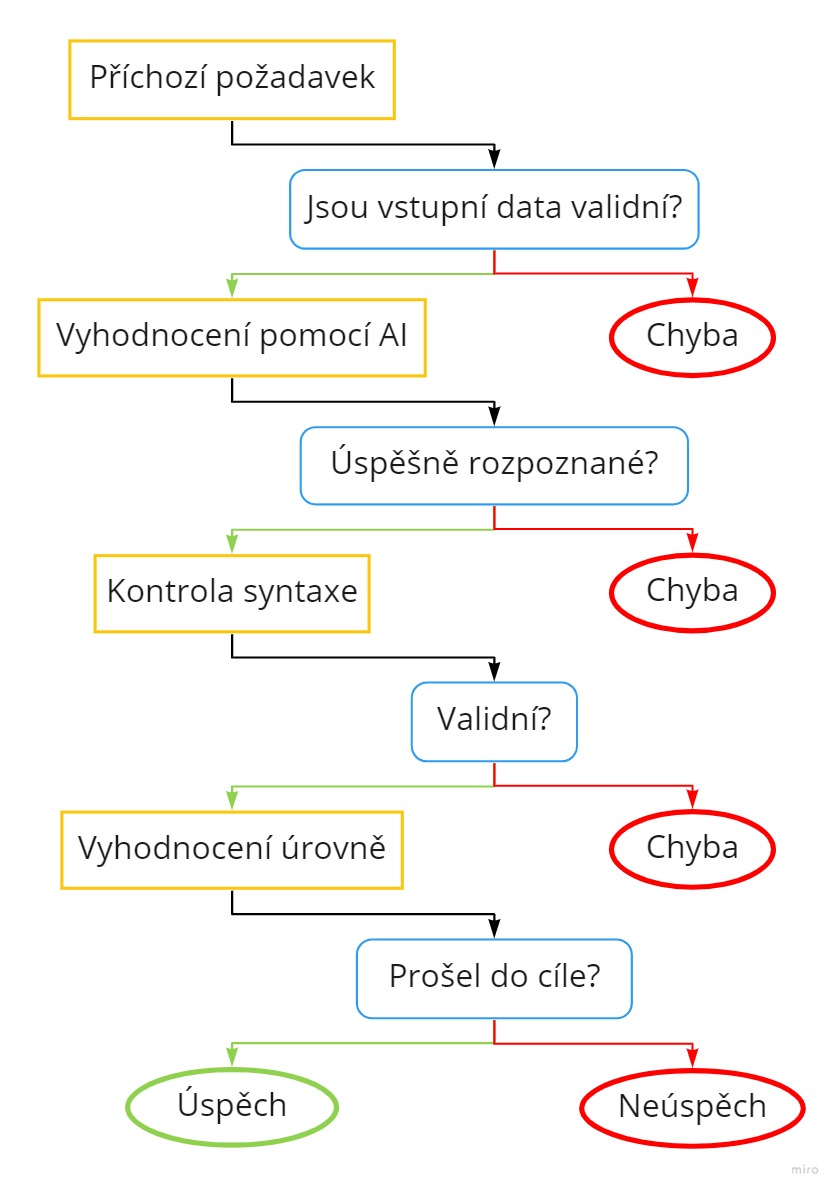
\includegraphics[width=0.3\textwidth]{img/proces.jpg}
    \caption{Proces vyhodnocování úrovně.}
    \label{fig:proces-vyhodnocovani}
\end{figure}

\subsubsubsection{Validace vstupů}
Před začátkem vyhodnocování je potřeba zkotrolovat, zda všechny údaje sedí. Pro úspěšnou validaci je potřeba zaslat číslo ostrova a úrovně, čas ve kterém se začínalo řešit a fotografie kartiček. Pro zkontrolování integrity času je použit hash, kterému musí sedět kontrolní součet. Kdyby ho uživatel nějak změnil, nebyl by potom tento čas validní.

\subsubsubsection{Vyhodnocení pomocí AI}
Po zvalidování vstupů je potřeba vyhodnotit data na obrázku. Pro tento účel slouží samostatný vyhodnocovací backend, na kterém běží Express.js a TensorFlow.js. Na tomto backendu je uložen vytrénovaný model pomocí Custom Vision od Microsoftu. Tento backend není veřejně přístupný a zavolat na něj může pouze hlavní backend.\par
Hlavní backend po přijetí obrázku zasílá tento obrázek na vyhodnocovací backned pomocí API rozhraní. Po úspěšném vyhodnocení jsou vráceny informace: jak jsou kartičky průměrně velké a pole, kde a s jakou přesností se konkrétní kartička nachází.

\subsubsubsection{Kontrola syntaxe a vyhodnocení úrovně}
Po vyhodnocení obrázku je provedena kontrola syntaxe a vyhodnocení úrovně.\par
Nejprve je potřeba zkontrolovat, zda rozpoznané kartičky obsahují \uv{Start} a \uv{Konec}. Dále je vypočítána přímka mezi těmito dvěma body a jsou získány kartičky které na této přímce leží (pomocí průměrné velikosti kartiček si lze vypočítat toleranci od přímky). Pak jsou pomocí pravého úhlu dopočítány přímky pro tyto kartičky a jsou k nim přiřazeny rozšiřující kartičky.\par
Když se někde vyskytne synkatická chyba (chybí kartička \uv{Start} nebo \uv{Konec}, kartička je na místě na kterém být nemůže) je hráři oznámeno, co udělal špatně a pokus je vyhodnocen jako neúspěšný.\par
Poslední částí je vyhodnocení úrovně. Pro tuto část je potřeba získat z databáze data o tom, jak úroveň vypadá. Server prochází úroveň krok po kroku a z toho zjišťuje jak si hráč vede. Nakonec server odesílá data o výsledku zpět do kontroléru a na frontend, kde se hráč dozví jak si vedl.

\subsubsection{Nasazení na server}
Nasazení na server je klíčový krok, který určuje zda je celá hra hratelná. Pro vytvoření vždy identického prostředí je potřeba votvořit kontejner, který obsahuje pouze data potřebná k běhu služby.\par
Pro vytvoření kontejnerů je použit Docker. Pomocí takzvaného \uv{Dockerfile} je zadefinován postup jak backend sestavit, který když následně sestavíme, dostaneme balík, který je možné kdekoliv sputit. Tento proces je vykonán jak u hlavního backendu, ale i u vyhodnocovacího backendu.\par
K následnému nasazení na server je použita platform Kubernetes, konkrétně K3s, která se stará o kontejnery, zajišťuje síťovou komunikaci a rozprostřívá zátěž mezi servery.
